\documentclass{beamer}
\usepackage[utf8]{inputenc}
\usepackage{subfig}
\usepackage{tabularx}
\usepackage{pgfpages}
\usepackage{array}
%---Propriétés presentation
\usetheme{Darmstadt}
%Pour ajouter un pied de page
\makeatletter
\setbeamertemplate{footline}
{
  \leavevmode%
  \hbox{%
  \begin{beamercolorbox}[wd=.333333\paperwidth,ht=2.25ex,dp=1ex,center]{author in head/foot}%
    \usebeamerfont{author in head/foot}\insertshortauthor%~~\beamer@ifempty{\insertshortinstitute}{}{(\insertshortinstitute)}
  \end{beamercolorbox}%
  \begin{beamercolorbox}[wd=.333333\paperwidth,ht=2.25ex,dp=1ex,center]{title in head/foot}%
    \usebeamerfont{title in head/foot}\insertshorttitle
  \end{beamercolorbox}%
  \begin{beamercolorbox}[wd=.333333\paperwidth,ht=2.25ex,dp=1ex,right]{date in head/foot}%
    \usebeamerfont{date in head/foot}\insertshortdate{}\hspace*{2em}
    \insertframenumber{} / \inserttotalframenumber\hspace*{2ex} 
  \end{beamercolorbox}}%
  \vskip0pt%
}
\makeatother
%\setbeameroption{show only notes}

%setbeameroption{show notes on second screen=left}




%Slide de titre
\title{PRD 48: Soutenance Intermédiaire}
\subtitle{Magic Portrait: Améliorons la photographie de portrait}
\author{Pierre-Yves Hervo \and Paul-François Jeau}
\date{04 décembre 2013}


\AtBeginSection[]
{
  \begin{frame}<beamer>{}
    \tableofcontents[currentsection]
  \end{frame}
}

\begin{document}



\begin{frame}
    \titlepage
    \begin{center}
        \begin{figure}
		    
\includegraphics[width=0.4\textwidth]{PolytechNantes}
        \end{figure}
        \textbf{Tuteur: Matthieu Perreira Da Silva\\
	            Coordinateur: José Martinez}
	\end{center}
	\note{PF: Bonjour nous vous remercions pour votre présence aujourd'hui. Cette soutenance se déroule dans le cadre des projets de recherche et développement. Notre sujet est le numéro 48 et s'intitule Magic Portrait Améliorons la photographie de portrait. Je vous présente PY et moi-même PY. Cette soutenance va retracer notre travail tout au long de cette première phase.}
\end{frame}

\begin{frame}{Plan}
    \tableofcontents
    \note{PF: En ce qui concerne la structure de cette prochaine demi-heure, nous aborderons 5 points:....}
\end{frame}

\section{Présentation du projet}

\subsection{Problématique générale}

\begin{frame}{Contexte et problématique}

\begin{itemize}
\item Sujet multimédia
\item Retouche des clichés en notre possession potentiellement compliquée
\item Connaissances nécessaires en photographie
\end{itemize}
\pause
\begin{block}{Problématique: }
Elle correspond à la question: que traiter et de quelle manière ?
\end{block}

\note{PF: Je vais à présent commencer par vous présenter le projet afin que les bases soient posés pour aborder les parties état de l'art et propositions. Tout d'abord notre porjet Magic portrait est résolument orienté multimédia puisqu'il est est lié à l'amélioration de photographie donc d'image. Pour le replacer dans son contexte, avec l'avénement et la démocratisation des appareils photos numériques, smarthphones, mais aussi des reseaux sociaux, beaucoup disposent de clichés à aposer en tant que photo de profil. Par photo de profil nous entendons photographie avec préponderance de visage de face. Ces photos pouvant être imparfaites, l'usage de logiciel de retouches ou l'appel aux compétences de professionnels sont des recours commun pour y rémedier. Mais cela induit un cout qui peut etre important, et dans le cas de l'acquisition de logiciel de retouche, il faut aussi des connaissances en photographie. Et tout le monde n'a pas la même fibre artistique et sens critique esthétique.}
\end{frame}

\subsection{Objectifs du projet}

\begin{frame}{Objectifs du projet}

\begin{itemize}
\item S'initier à la recherche
\item Appliquer la méthodologie au domaine la photographie de portrait
\item Déterminer des critères discriminants la qualité des photographies
\item Déterminer les techniques existantes de correction
\item Proposer des solutions possibles d'amélioration dans ce domaine
\end{itemize}

\note{PF: Les objectifs découlant sont donc variés, avec un premier basé sur l'initiation à la recherche. Dans notre cas, je le repete le domaine parcouru est celui de la photographie de portrait. Afin de répondre à la problématique, il nous faut répondre lors de ce projet à deux axes, étudier les critères utilisés lors de l'évaluation de l'esthétisme des photographies mais aussi nous intéresser aux méthodes d'amélioration qui sont disponibles actuellement}
\end{frame}



\section{Etat de l'art}

\subsection{Les critères esthétiques}

\begin{frame}{Les critères de haut niveau}

\begin{itemize}
\item Étude de 14 critères esthétiques assez subjectifs
\item 3 catégories de critères: composition, contenu, autres
\item Profondeur de champ, type de scène, luminosité du ciel
\item Certains spécifiques au cas des portraits
\end{itemize}

\end{frame}

\begin{frame}{Les critères de haut niveau}

\begin{figure}[htp]
 \centering
 \subfloat[Photo d'un Amateur]{\label{fig:photoama}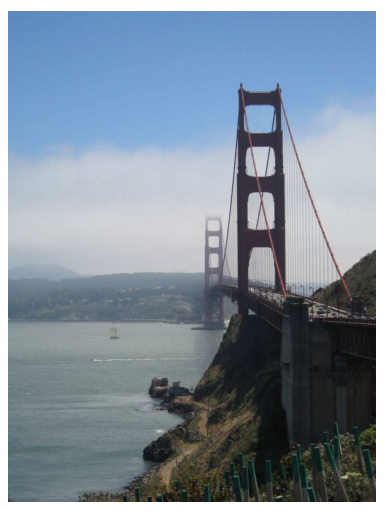
\includegraphics[scale=0.3]{ea_photo_ama}}               
 \subfloat[Photo d'un Professionnel]{\label{fig:photopro}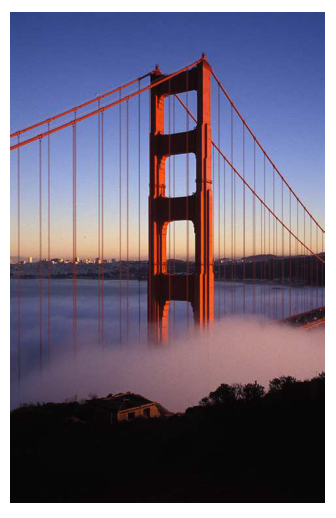
\includegraphics[scale=0.30]{ea_photo_pro}}
 \caption{Comparaison entre la photo d'un amateur et celle d'un professionnel, Ke et Al.}
 \label{fig:ComparaisonPhotosAmateurPro}
\end{figure}

\end{frame}

\begin{frame}{Comparatif}

\begin{table}
\caption{Comparaison de certains critères de haut niveau}
\begin{tabular}{|p{2.5cm}|p{3cm}|p{1.5cm}|p{2cm}|}
\hline
\textbf{Critère} & \textbf{Utilisation} & \textbf{Simplicité  calcul} & \textbf{Impact de la qualité de l'image} \\ \hline
Règle des Tiers & Mise en valeur du sujet principal & Difficile & Peu \\ \hline
Profondeur de champ & Mise en valeur du sujet principal & Moyenne & Oui \\ \hline
Couleurs complémentaires & Rendu plus professionnel & Moyenne & Oui(fort bruit) \\ \hline
Taille du visage & Prépondérance du visage & Simple & Non \\ \hline
\end{tabular}
\label{ComparaisonHautNiveau}
\end{table}

\end{frame}

\begin{frame}{Les critères de bas niveau}

\begin{itemize}
\item Critères plus objectifs
\item Mesure du flou de l'image, saturation globale, teinte générale, 
\item Calcul des mesures dans d'autres espaces de couleurs comme le HSV
\end{itemize}

\end{frame}

\begin{frame}{Comparatif}

\begin{table}
\caption{Comparaison de certains critères de bas niveau}
\begin{tabular}{|p{3cm}|p{2.5cm}|p{1.5cm}|p{2cm}|}
\hline
Critère & Utilisation & Simplicité  calcul & Impact de la qualité de l'image \\ \hline
Histogramme de la couleur de l'image & Coloration de l'image & Simple & Oui \\ \hline
Propriétés de Haar & Détecter les visages & Difficile & Non \\ \hline
Mesure du flou & Netteté de l'image & Moyenne & Oui \\ \hline
Carte de contraste multi-échelle & Détecter les objets & Difficile & Peu \\ \hline
Luminosité & Niveau d'exposition & Simple & Oui \\ \hline
\end{tabular}
\label{ComparaisonBasNiveau}
\end{table}

\end{frame}

\subsection{Les méthodes d'amélioration des photographies de portrait}

\begin{frame}{Les méthodes globales}
\begin{itemize}
\item 2 méthodes
\item Une par lissage de la peau
\item L'autre par déformation du visage
\end{itemize}
\note{PF: Merci, je vais ainsi vous faire part de nos études sur les méthodes d'ameliorations des portraits, à commencer par les méthodes que nous avons qualifiées de globales. Nous en avons étudié deux, l'une était dédiée à tout ce qui a trait à la peau, la seconde ameliorait une image en déformant la structure du visage}
\end{frame}

\begin{frame}{Technique globale pour l’amélioration de la peau}
\begin{figure}
	\centering
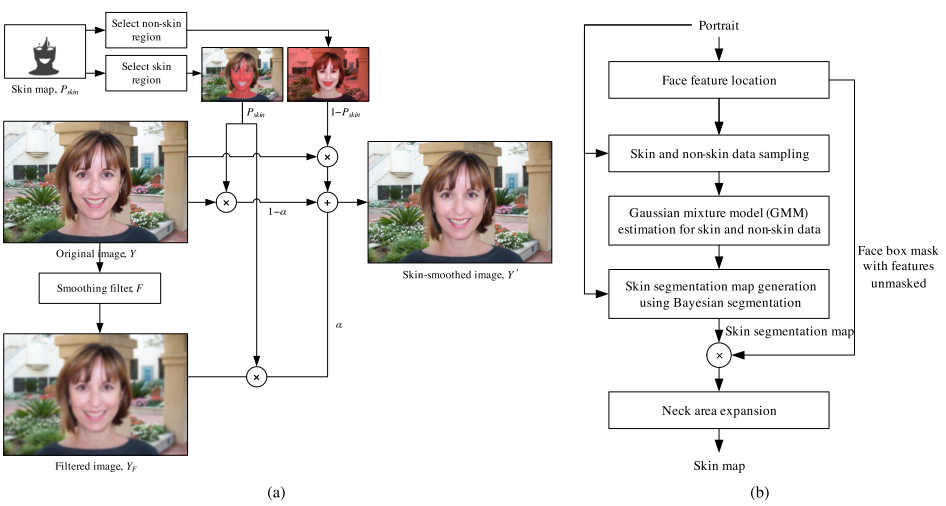
\includegraphics[width=0.9\textwidth]{ea_algo_smoothing}
	\caption{Principe de fonctionnement de la méthode développée par Lee et Al.}
	\label{fig:FonctionnementLee}
\end{figure}
\note{PF: i nous nous concentrons sur la méthode de Lee dédiée à la retouche globale de la peau, voici le schéma de la méthode issu de l'article. Les pixels de peau sont au préalables détectés et vont alimenter un masque de pixels de peau. On peut donc obtenir par différence les pixels qui ne relevent pas de la peau. Dans une seconde partie, on applique un flou gaussien sur l'image originale. Dans l'image finale, on combine les valeurs des pixels de peau originales avec celles tirées de l'image flouttée (avec un certain coefficient pour que la peau garde un certain niveau de détails). Les autres pixels sont ceux de l'image originale, il n'y a donc pas de changement du fond ni des yeux et de la bouche. On conserve donc leur détails, mais si le fond est trop chargé, compliqué, le sujet ressort mal. Avec cette méthode sont donc adoucies les rides, les rougeurs sont estompées,...}
\end{frame}

\begin{frame}{Méthode d’amélioration globale de portrait par déformation du visage}
\begin{figure}
	\centering
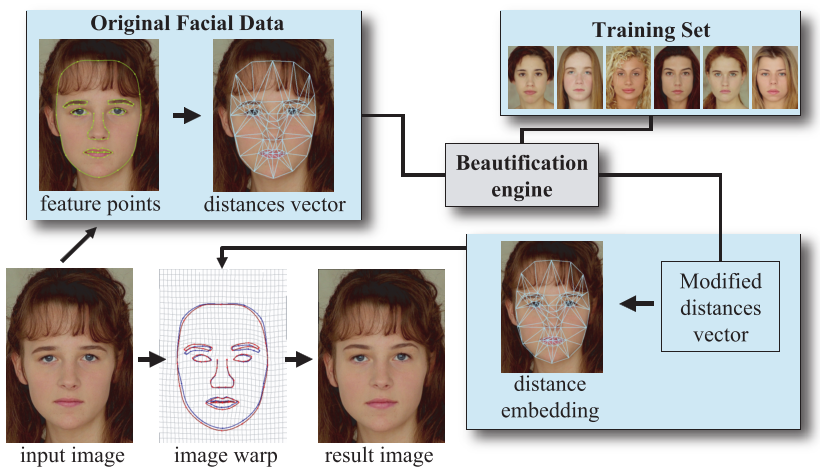
\includegraphics[width=0.8\textwidth]{ea_algo_datadriven}
	\caption{Principe de fonctionnement de la méthode développée par Leyvand et Al.}
	\note{PF: Dans le cas de la seconde méthode de Leyvand, la cible est toute autre, puisque l'on ne cherche à modifier que la structure du visage. L'algorithme détecte tout d'abord le visage et les points caractéristiques. On peut ensuite construire un graphe de distances à partir de la carte du visage.
A partir de sa base de graphe de vecteurs distances obtenus sur des visages qualifié de beau, le masque le plus proche est retourné. Le visage original est ensuite déformé pour épouser la forme du masque le plus proche. Ici on constate que les sourcils sont plus courbés, et que le visage semble plus souriant. Cette méthode permet d'obtenir de bons rendus pour des sujets adultes mais ce n'est pas possible pour les enfants si la base ne possede pas des visages de la meme categorie. De plus dans ses limites, on peut se demander si réinterpreter la structure du visage ne va pas un peu loin. La méthode ne corrige pas la peau ou les imperfections, l'embellissement est exclusivement fait par déformation }
\end{figure}
\end{frame}


\begin{frame}{Les méthodes locales}
\begin{itemize}
\item 3 méthodes étudiées 
\item Un mode de traitement par lots
\item Sur des sous-régions du visage 
\item La dernière par filtrage itératif
\end{itemize}
\note{Je vais passer au cas des méthodes locales. Nous en avons étudié 3....}
\end{frame}

\begin{frame}{Méthode d’amélioration des photos de portrait par enchainement de traitements sur différentes imperfections}
\begin{itemize}
\item Déposée par Matraszek et Simon
\item Traitement par lots
\item Permet de choisir la dose de correction
\item 4 zones modifiables : les yeux, la peau, la bouche, les dents
\item Algorithme : détection puis traitement correctif sur chaque zone
\end{itemize}
\note{PF: cette méthode a été déposée dans un brevet qui depose un logiciel de retouche combinables sur une photographie. Pour ce qui est du fonctionnement, la détection du visage est à realisé afin d'extraire les zones caracteristiques du visage. Pour chacune des zones peau , yeux, nez, bouche, sourcils, cou, cheveux un traitement a été développé. L'utilisateur peut agir sur 4 zones de la photo, sinon le logiciel peut corriger dans l'ordre la teinte de la peau, de la blancheur des dents et des yeux. Il termine par une modification de la structure du
visage. La technique n'est pas exploitable mais elle nous a permis de constater que les zones des sourcils, des cheveux ont pu être detectées. }
\end{frame}

\begin{frame}{Méthode d’amélioration des photos de portrait sur des sous-régions du visage}
\begin{itemize}
\item Déposée par Ciuc et Al.
\item But: améliorer la blancheur des yeux et des dents
\item Suppression du bruit puis correction de la luminance
\item Passage dans l'espace colorimétrique YUV
\end{itemize}
\note{dans cette deuxieme methode, les retouches sont recherchées et realisées exclusivement dans des sous regions du visage , yeux et bouches. C'est la blancheur des yeux et des dents qui sont corrigées par traitement de la luminance. Pour augmenter la blancheur des
dents, c’est la composante Y qui se voit augmentée, et
les valeurs absolues des composantes U et V sont diminuées.
Si elle est trop forte, la luminance va être répartie
via l’application d’un flou. La peau est aussi un peu traitée en termes de couleur mais seulement dans le voinage des regions des yeux et de la bouche.}
\end{frame}

\begin{frame}{Technique d’amélioration plus fine basée sur l’analyse des défauts du portrait}
\begin{itemize}
\item Déposée par Konoplev
\item Passe de l'espace RGB vers CIELAB
\item Filtre de détection du bruit avec de multiples paramètres
\item Filtre itératif, le niveau de bruit est modifié à chaque étape
\end{itemize}
\note{PF: Cette dernière méthode de Konoplev est basée sur le passaged en CIELAB: modèle de représentation des couleurs
développé en 1976 par la Commission internationale de l’éclairage
(CIE) 11. La composante L correspond à la clarté, a et b désigne les
gammes de couleurs, afin de disposer d'un espace de couleurs plus naturel. La méthode ressemble à la premiere, à la différence ou elle utilise un meme filtre sur les différentes imperfections mais avec des parametres différents pour accentuer plus ou moins la retouche. La aussi les zones retouchées sont les rides, acnée, bruit, rougeur. Le plus de la méthode est aussi la correction des contrastes et luminosité de l'image. Afin de conserver un bon niveau de détails, des pixels de l'image originale sont reinjectés à la fin.}
\end{frame}


\begin{frame}{Comparatif}
\begin{table}
\caption{Comparaison des Méthodes d'Amélioration}
\begin{tabular}{|p{3cm}|p{3cm}|p{3.5cm}|}
\hline
Méthode & Zones traitées & Principe général \\ \hline
Pour la peau & Peau & Application de flou \\ \hline
Par déformation du visage & Forme du visage & Moteur d'embellissement par apprentissage \\ \hline
Par enchaînement de traitements & Rides, Acné, Rougeurs, Bruit & Traitements dédiés \\ \hline
Sur des sous-régions du visage & Dents, yeux, bouche & Sur des sous-régions  \\ \hline
Analyse des défauts du portrait & Contraste, Luminosité, Rides, Rougeurs & Traitements dédiés, combinaison \\ \hline
\end{tabular}
\label{ComparaisonMethodes}
\end{table}

\end{frame}



\section{Propositions}
\subsection{Proposition 1}
\begin{frame}{Extension de la méthode de Lee et Al.}
\begin{itemize}
\item Choix de ne pas utiliser une technique qui déforme le visage
\item Deux niveaux de traitement
\end{itemize}
\begin{enumerate}
\item Traitement du fond, domaine inexploité avec ajout de profondeur de champ
\item Lissage du visage pour corriger les imperfections cutanées
\end{enumerate}
\end{frame}
\subsection{Proposition 2}
\begin{frame}{Méthode de traitement optimale}
\begin{itemize}
\item Complément de la proposition 1
\item Consiste à traiter les yeux et les cheveux en suppléments 
\end{itemize}
\end{frame}
\subsection{Choix de la proposition}
\begin{frame}{Comparaison des propositions}

\begin{center}
\begin{figure}
    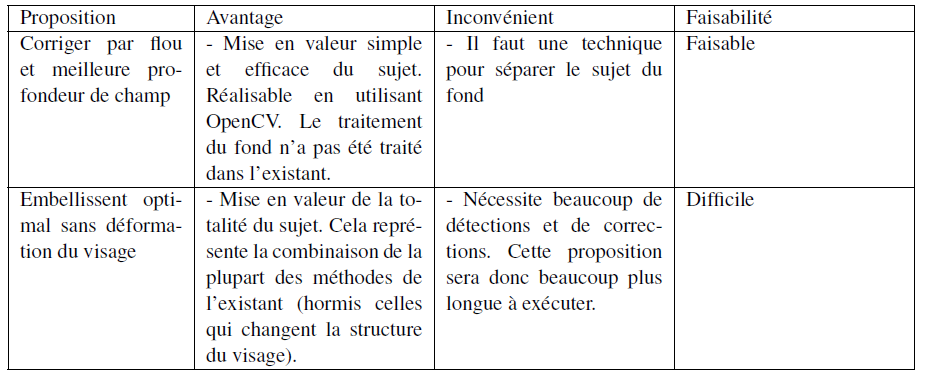
\includegraphics[width=1.0\textwidth]{TableauCompProp}
	\caption{Tableau comparatif des propositions possibles}
	\label{fig:tabcompprop}
\end{figure}
\end{center}
\end{frame}


\section{Planification}
\subsection{Planification}
\begin{frame}{Planning prévisionnel}
\begin{figure}
	\centering
		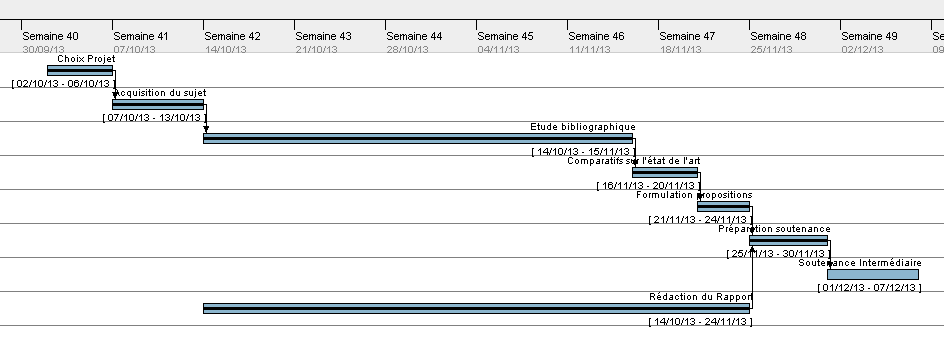
\includegraphics[width=0.95\textwidth]{p1_previsionnel}
	\caption{Planification prévisionnelle}
	\label{fig:PlanningPrevisionnel}
\end{figure}
\end{frame}
\begin{frame}{Planning effectif}
\begin{figure}
	\centering
		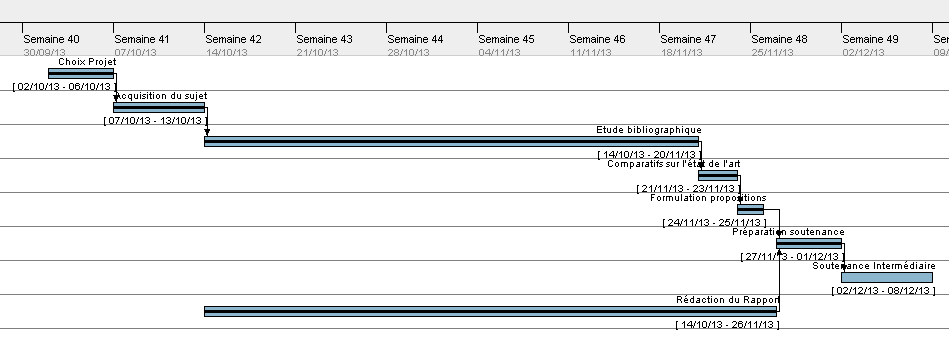
\includegraphics[width=0.95\textwidth]{p1_effectif}
	\caption{Planification effective}
	\label{fig:PlanningEffectif}
\end{figure}
\end{frame}
\begin{frame}{Comparaison des plannings}
\begin{figure}
	\centering
		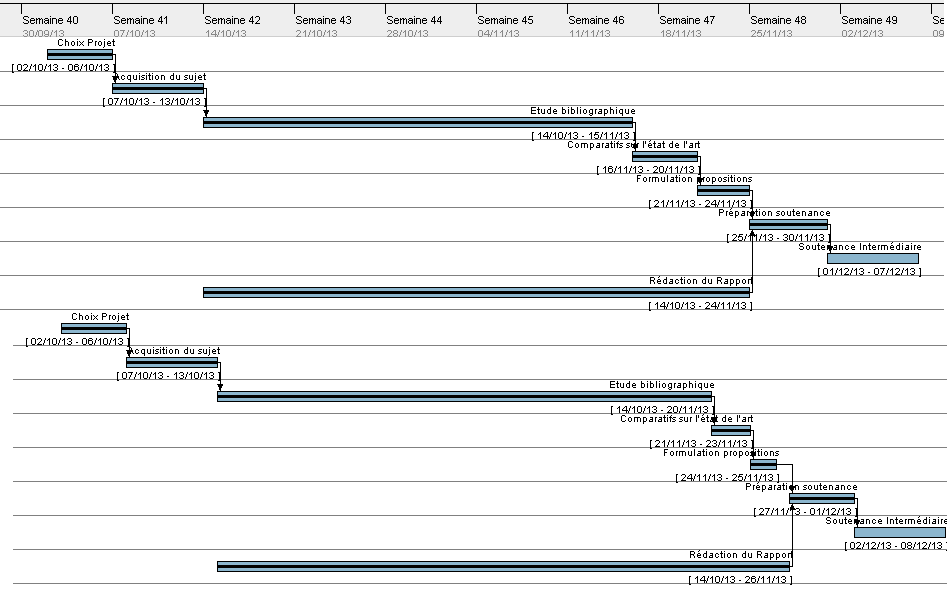
\includegraphics[width=0.95\textwidth]{p1_previ_effe}
	\caption{Comparaison des plannings}
	\label{fig:PlanningEffePrevi}
\end{figure}
\end{frame}


\begin{frame}{Prochaine phase}
\begin{itemize}
\item 7 semaines restantes hors préparation et soutenance finale
\item Formaliser la conception de la proposition choisie
\item Mettre en œuvre la solution
\end{itemize}
\end{frame}

\section{Conclusion}
\begin{frame}{Conclusion}
\begin{itemize}
\item Connaissances des critères principalement retenus pour les évaluations
\item Étude de méthodes d'amélioration existantes
\item Proposition étendant les traitements au fond de la photographie 
\end{itemize}
\end{frame}

\begin{frame}{Sources}
\begin{itemize}
\item Les articles évoqués et les images utilisées figurent dans la bibliographie du rapport 
\end{itemize}
\end{frame}

\end{document}
